\usepackage{array}
\usepackage{tikz}
\usetikzlibrary{arrows.meta}
\usepackage{listings}

% Named colors for literate replacements (avoid ! in \lstset literals).
\colorlet{lstkw}{blue!70!black}
\colorlet{lstkwii}{violet!75!black}
\colorlet{lstflag}{teal!70!black}
\colorlet{lststr}{orange!85!black}
\colorlet{lsthdr}{blue!70!black}
\colorlet{lstcmt}{black!55}

% --- Shared framed block ---
\lstdefinestyle{mcpblock}{%
  basicstyle=\ttfamily\footnotesize,
  keywordstyle=\bfseries\color{lstkw},
  commentstyle=\itshape\color{lstcmt},
  stringstyle=\color{lststr},
  columns=fullflexible,
  keepspaces=true,
  tabsize=2,
  showstringspaces=false,
  breaklines=true,
  breakatwhitespace=true,
  frame=single,
  rulecolor=\color{black!35},
  backgroundcolor=\color{black!4},
  xleftmargin=0.5em,
  xrightmargin=0.5em,
  aboveskip=4pt,
  belowskip=4pt,
}

% --- Inline (no frame) ---
\lstdefinestyle{inline}{%
  basicstyle=\ttfamily\small,
  showstringspaces=false,
}

% --- JSON / JSON-RPC ---
\lstdefinelanguage{JSONRPC}{%
  morestring=[b]",%
  sensitive=false,%
  morecomment=[l]{//},%
  morekeywords={true,false,null},%
  morekeywords=[2]{jsonrpc,method,params,result,id,error},%
}
\lstdefinestyle{json}{%
  style=mcpblock,
  language=JSONRPC,
  keywordstyle=\bfseries\color{lstkw},
  keywordstyle=[2]\color{lstkwii},
  stringstyle=\color{lststr},
}

% --- Bash / shell (extends listings bash: commands, flags, npm scopes) ---
\lstdefinelanguage{shellcmd}[]{bash}{%
  morekeywords={npx,npm,uvx,pip,uv,python,node,curl,git,docker,run},%
  morekeywords=[2]{-y,-m,-f,-v,-h,-p,--help,--directory,--version},%
  morestring=[b]',%
  sensitive=false,%
}
\lstdefinestyle{bash}{%
  style=mcpblock,
  language=shellcmd,
  keywordstyle=\color{lstkwii},
  keywordstyle=[2]\color{lstflag},
  commentstyle=\color{lstcmt},
  stringstyle=\color{lststr},
  literate={@}{{\textcolor{lststr}{@}}}1,
}

% --- Python ---
\lstdefinestyle{python}{%
  style=mcpblock,
  language=Python,
}
\lstdefinestyle{pythoninline}{%
  language=Python,
  basicstyle=\ttfamily\small,
  keywordstyle=\bfseries\color{lstkw},
  commentstyle=\itshape\color{lstcmt},
  stringstyle=\color{lststr},
  columns=fullflexible,
  keepspaces=true,
  showstringspaces=false,
}

% --- Java ---
\lstdefinestyle{java}{%
  style=mcpblock,
  language=Java,
}
\lstdefinestyle{javainline}{%
  language=Java,
  basicstyle=\ttfamily\small,
  keywordstyle=\bfseries\color{lstkw},
  commentstyle=\itshape\color{lstcmt},
  stringstyle=\color{lststr},
  columns=fullflexible,
  keepspaces=true,
  showstringspaces=false,
}

% --- JavaScript / Node.js ---
\lstdefinestyle{js}{%
  style=mcpblock,
  language=JavaScript,
}
\lstdefinestyle{jsinline}{%
  language=JavaScript,
  basicstyle=\ttfamily\small,
  keywordstyle=\bfseries\color{lstkw},
  commentstyle=\itshape\color{lstcmt},
  stringstyle=\color{lststr},
  columns=fullflexible,
  keepspaces=true,
  showstringspaces=false,
}

% --- HTTP trace (headers + body in exchange diagrams) ---
\lstdefinelanguage{httptrace}{%
  alsoletter={-./},%
  morekeywords={GET,POST,HTTP,OK,Accepted},%
  morekeywords=[2]{Host,Accept,Content-Type,event,data},%
  sensitive=false,%
}
\lstdefinestyle{http}{%
  basicstyle=\ttfamily\footnotesize,
  language=httptrace,
  keywordstyle=\bfseries\color{lstkwii},
  keywordstyle=[2]\color{lsthdr},
  frame=single,
  framerule=0.4pt,
  rulecolor=\color{black!35},
  backgroundcolor=\color{black!4},
  framesep=3pt,
  xleftmargin=2pt,
  xrightmargin=2pt,
  breaklines=true,
  breakatwhitespace=true,
  columns=fullflexible,
  keepspaces=true,
  showstringspaces=false,
  aboveskip=4pt,
  belowskip=4pt,
}

% --- Side-by-side request / response ---
\tikzset{%
  http@arrow/.style={%
    -{Stealth[scale=0.88]}, semithick, shorten >=0.5pt, shorten <=0.5pt, draw=black!55},
}
\newenvironment{httpexchange}{%
  \par\addvspace{\baselineskip}%
  \begingroup
  \hfuzz=30pt\relax
  \begin{center}%
  \noindent
  \begin{tabular}{@{} m{0.4\linewidth} >{\centering\arraybackslash}m{1.28cm} m{0.4\linewidth} @{}}%
}{%
  \end{tabular}%
  \end{center}%
  \endgroup
  \par\addvspace{\baselineskip}%
}
\newcommand{\httpmidarrows}{%
  &
  \begin{minipage}[c]{1.28cm}%
    \centering
    \normalfont\footnotesize REQ\par\vspace{1pt}%
    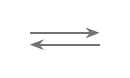
\begin{tikzpicture}[x=1cm, y=0.75cm]
      \draw[http@arrow] (0,0.1) -- (0.92,0.1);
      \draw[http@arrow] (0.92,-0.1) -- (0,-0.1);
    \end{tikzpicture}\par\vspace{1pt}%
    \normalfont\footnotesize RESP%
  \end{minipage}%
  &
}
